% !TEX program = xelatex
\documentclass[10pt,letterpaper,twocolumn]{article}
\usepackage[margin=0.75in]{geometry}
\usepackage{fontspec}
\setmainfont{Latin Modern Roman}[Extension=.otf,UprightFont=lmroman10-regular,BoldFont=lmroman10-bold,ItalicFont=lmroman10-italic,BoldItalicFont=lmroman10-bolditalic]
\setsansfont{Latin Modern Sans}[Extension=.otf,UprightFont=lmsans10-regular,BoldFont=lmsans10-bold,ItalicFont=lmsans10-oblique]
\setmonofont{Latin Modern Mono}[Extension=.otf,UprightFont=lmmono10-regular,Scale=0.85]
\newfontfamily\acbold{ywft-processing-bold}[Path=../../system/public/type/webfonts/,Extension=.ttf]
\usepackage{xcolor,titlesec,booktabs,tabularx,enumitem,fancyhdr,microtype,tikz,balance}
\usepackage[numbers,sort&compress]{natbib}
\usepackage{hyperref,xurl}
\usepackage{../ac-source-bundle}
\usetikzlibrary{positioning,arrows.meta}
\definecolor{acpink}{RGB}{180,72,135}
\definecolor{acpurple}{RGB}{120,80,180}
\definecolor{acdark}{RGB}{64,56,74}
\definecolor{acgray}{RGB}{119,119,119}
\definecolor{acgreen}{RGB}{35,105,85}
\definecolor{aclightgray}{RGB}{244,243,246}
\newcommand{\acdot}{{\color{acpink}.}}
\newcommand{\ac}{Aesthetic{\acdot}Computer}
\newcommand{\code}[1]{\texttt{\nolinkurl{#1}}}
\hypersetup{colorlinks=true,linkcolor=acpurple,urlcolor=acpurple,citecolor=acpurple,pdftitle={Rollback Over a Relay},pdfauthor={@jeffrey}}
\titleformat{\section}{\normalfont\bfseries\normalsize\uppercase}{\thesection.}{0.5em}{}
\titlespacing{\section}{0pt}{1em}{0.3em}
\titleformat{\subsection}{\normalfont\bfseries\small}{\thesubsection}{0.5em}{}
\titlespacing{\subsection}{0pt}{0.7em}{0.2em}
\pagestyle{fancy}\fancyhf{}\renewcommand{\headrulewidth}{0pt}
\fancyfoot[C]{\footnotesize\thepage}
\setlength{\columnsep}{1.8em}\setlength{\parskip}{0.25em}
\setlist[enumerate]{nosep,leftmargin=1.4em}
\newcolumntype{L}{>{\raggedright\arraybackslash}X}
\renewcommand{\dbltopfraction}{0.9}\renewcommand{\topfraction}{0.9}
\renewcommand{\textfraction}{0.08}
\setcounter{dbltopnumber}{2}
\emergencystretch=1.4em
\begin{document}
\twocolumn[{
\begin{center}
{\acbold\fontsize{24}{28}\selectfont\color{acdark} Rollback Over a Relay}\par
\vspace{0.4em}
{\large\color{acdark} How oskiewar and dool share a fight, and what the tests said on November 8}\par
\vspace{0.7em}
\href{https://prompt.ac/@jeffrey}{@jeffrey}\par
{\small \ac{} · November 8, 2026}\par
{\small ORCID: \href{https://orcid.org/0009-0007-4460-4913}{0009-0007-4460-4913}}
\end{center}
\begin{quote}\small\noindent\textbf{Abstract.}
Two games inside \ac{} move a shared world between players in two different ways. Oskiewar, a two-seat fighting game, runs the whole fight on both machines: each seat schedules its own pad two frames ahead, mails it with ten frames of redundancy through a small relay that forwards seat to seat and nothing else, predicts the rival's missing pad, and rewinds to a snapshot when the real one disagrees. dool, the two-player world under the \ac{} homepage, keeps one authoritative server at 60~Hz, lets the client predict only its own body from unacknowledged commands, and interpolates everyone else. This report describes both designs from the source, the relay that carries the rollback lane (a WebSocket for everything that must arrive and a UDP or WebRTC datagram lane for the one kind of traffic that should not wait), the regional relays that halved a Los Angeles round trip, and the test record taken today: the relay suite passes 43 of 43, dool's suite 64 of 64, and the rollback suite 26 of 42, with every synchronization assertion green and the sixteen failures in gameplay fixtures that were already red at the test file's last commit. It is written to hand to a peer for review, and closes with the questions worth their time.
\end{quote}\vspace{0.5em}
}]

\section{Two games, two answers}\label{sec:problem}
A fighting game and a build-and-walk world want different things from the network. In a fight, the thing that hurts is the time between a press and its consequence on the other screen; thirty milliseconds is a display's own lag and a hundred is a different game. In a room where people walk, talk, carry objects and ask an agent to build, the thing that hurts is disagreement: two people must see the same object in the same place, and somebody has to be right about who picked it up.

Oskiewar answers the first problem the way modern fighting games do \citep{ggpo,sf6}: both machines simulate everything, and the network carries only inputs. dool answers the second the way shooters have since Quake: one server simulates, clients send intentions and draw what they are told, with a little local prediction so the hand feels attached \citep{gaffer,valve}. Both ride the same infrastructure family, Node servers behind Caddy on DigitalOcean, and both are small enough to read in an afternoon. Section~\ref{sec:relay} describes the relay, Section~\ref{sec:rollback} the rollback lane on top of it, Section~\ref{sec:dool} dool's room, Section~\ref{sec:evidence} today's test record, and Section~\ref{sec:questions} what a reviewer could usefully poke at.

\begin{figure*}[t]
\centering
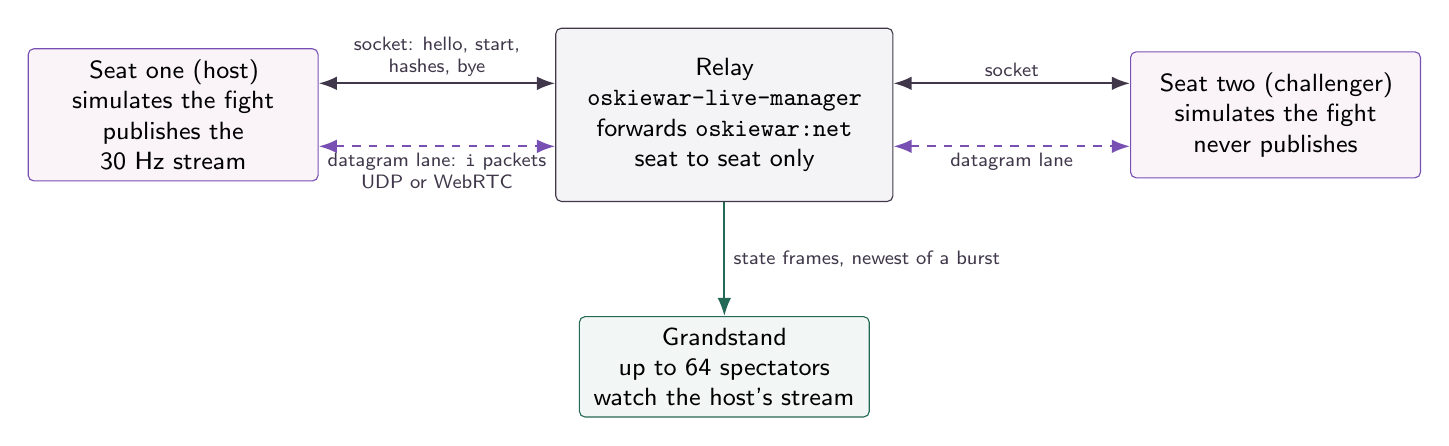
\begin{tikzpicture}[>=Latex,
 seat/.style={draw=acpurple,rounded corners=2pt,align=center,font=\sffamily\small,minimum height=16mm,text width=34mm,inner sep=4pt,fill=acpink!6},
 relay/.style={draw=acdark,rounded corners=2pt,align=center,font=\sffamily\small,minimum height=22mm,text width=40mm,inner sep=4pt,fill=aclightgray},
 stand/.style={draw=acgreen,rounded corners=2pt,align=center,font=\sffamily\small,minimum height=12mm,text width=34mm,inner sep=4pt,fill=acgreen!6},
 ws/.style={<->,thick,draw=acdark},
 dg/.style={<->,thick,dashed,draw=acpurple},
 pub/.style={->,thick,draw=acgreen},
 lbl/.style={font=\sffamily\scriptsize,text=acdark,align=center,inner sep=1pt}]
\node[seat] (host) at (0,0) {Seat one (host)\\simulates the fight\\publishes the 30 Hz stream};
\node[relay] (relay) at (7.0,0) {Relay\\\code{oskiewar-live-manager}\\forwards \code{oskiewar:net}\\seat to seat only};
\node[seat] (guest) at (14.0,0) {Seat two (challenger)\\simulates the fight\\never publishes};
\node[stand] (stand) at (7.0,-3.2) {Grandstand\\up to 64 spectators\\watch the host's stream};
\draw[ws] ([yshift=4mm]host.east) -- node[lbl,above=1pt] {socket: hello, start,\\hashes, bye} ([yshift=4mm]relay.west);
\draw[ws] ([yshift=4mm]relay.east) -- node[lbl,above=1pt] {socket} ([yshift=4mm]guest.west);
\draw[dg] ([yshift=-4mm]host.east) -- node[lbl,below=1pt] {datagram lane: \code{i} packets\\UDP or WebRTC} ([yshift=-4mm]relay.west);
\draw[dg] ([yshift=-4mm]relay.east) -- node[lbl,below=1pt] {datagram lane} ([yshift=-4mm]guest.west);
\draw[pub] (relay.south) -- node[lbl,right=2pt] {state frames, newest of a burst} (stand.north);
\end{tikzpicture}
\caption{The oskiewar topology. Both seats run the simulation; the relay forwards each seat's small \code{oskiewar:net} packets to the other and to nobody else. Input packets, which carry their own redundancy, may take the unreliable datagram lane once a seat has presented its token; the deal, state hashes and goodbyes stay on the socket. The host still publishes a 30~Hz state stream for spectators, which the challenger never watches.}
\label{fig:topology}
\end{figure*}

\section{The relay}\label{sec:relay}
\subsection{One manager, many places}
The relay is one class, \code{OskiewarLiveManager}, in \code{session-server/oskiewar-live-manager.mjs} (1,432 lines at core revision \code{f2d1f744c2}). The session-server monolith in New Jersey mounts it at \code{/oskiewar-live}; \code{oskiewar-relay.mjs} runs the same class on its own, with nothing beside it, so a second copy can stand wherever players are. On October 14 a copy went up in DigitalOcean's \code{sfo3} region as \code{relay-sfo.aesthetic.computer}. Through a relay a fight's round trip is each player's round trip to it added together, and two Los Angeles players measured 193~ms through New Jersey against 64~ms through San Francisco \citep{westcoast}. The game's \code{round-room.mjs} asks every relay whether it already hosts a room and otherwise picks the one that answers \code{/oskiewar-ping} fastest; a room lives on exactly one relay and both players must share it. No directory exists; two hosts are listed in the client.

\code{relay/deploy-relay.sh} turns a fresh Ubuntu droplet into a relay: Node~22, the relay under systemd on loopback port 8890, Caddy terminating TLS with an automatic certificate, and firewall holes for UDP 8891 and the WebRTC port range. Rerunning it copies four files and restarts the service. The relay needs nothing else from the repository, which is the property that makes it portable to somebody else's box.

\subsection{What the relay checks and what it leaves alone}
Everything the relay accepts is bounded: a 2~KiB cap on \code{oskiewar:net} packets, a 16~KiB cap on published state frames, closed key sets and integer ranges on every field it validates (\code{validateOskiewarLiveState}, \code{validateOskiewarFfaState}), a 15~ms floor between held-pad packets on the older streamed lane, 64 spectator seats plus a small allowance for agents. The relay never rate-limits the rollback lane, because a dropped input packet is a rollback the other seat has to eat. It also does not read the rollback packets. \code{relayNet} checks that the payload is a small JSON object and that the sender holds a seat, then hands the packet to the other seat. What the two games say to each other is theirs.

\subsection{The datagram lane}
Over a WebSocket a lost packet holds every packet behind it until TCP has resent it. One drop on a phone's Wi-Fi froze the rival's presses for a round trip or two, and the rollback lane ate the stall as a burst of mispredictions. Input packets already carry the last ten frames, so a lost one is covered by the next; they are the one kind of traffic that wants UDP. Since October 15 each seat is handed a random 96-bit token on its socket (\code{oskiewar:udp}). Whatever presents that token over a datagram path, a raw UDP socket from the Mac app or a geckos.io WebRTC data channel from a browser, becomes that seat's endpoint. The relay sends to an endpoint only after it has presented a live token and only while it has spoken in the last 1.5~s; otherwise the rival's packets fall back to the socket. Nothing is ever sent to an address that has not spoken first, so the relay cannot be aimed at a third party. Only \code{i} packets without a state hash take the lane (\code{laneEligible}); the deal, hashes and goodbyes stay on the socket. The San Francisco relay's health endpoint reported, at the time of writing, 117,222 datagrams in, 117,081 out and 100 refused since its last restart, at commit \code{5a08d88c47}.

\section{The rollback lane}\label{sec:rollback}
\subsection{Shape}
Both seats run the same program from the same frame zero. Each schedules its own pad \code{NET\_INPUT\_DELAY} frames ahead, mails every pad it has decided on, simulates the current frame with the rival's last known pad standing in for one that has not arrived, and on a contradiction restores the snapshot of the frame before the wrong guess and re-simulates forward in silence. Table~\ref{tab:constants} gives the constants and the reasoning the source records beside each one.

\begin{table}[t]
\centering\small
\begin{tabularx}{\columnwidth}{@{}l r L@{}}
\toprule
constant & value & why \\
\midrule
\code{NET\_INPUT\_DELAY} & 2 frames & 33~ms at 60~Hz, a display's own lag; a rival packet inside it costs no rollback \\
\code{NET\_MAX\_ROLLBACK} & 8 frames & 133~ms of one-way silence, past the relay's p99; beyond it a seat holds instead of guessing \\
\code{NET\_REDUNDANCY} & 10 frames & every packet re-sends ten pads, so loss recovery needs no ack protocol \\
\code{NET\_HASH\_EVERY} & 30 frames & a state hash rides out twice a second at the newest frame both pads are known for \\
\code{NET\_PEER\_LOST\_MS} & 4000 & wall-clock silence after which the rival is gone \\
\code{NET\_DESYNC\_COOLDOWN\_MS} & 60000 & after a desync, no new rollback session for a minute \\
\code{MAX\_NET\_BYTES} (relay) & 2048 & the cap on one \code{oskiewar:net} packet \\
\code{LANE\_FRESH\_MS} (relay) & 1500 & how long a datagram endpoint is trusted after it last spoke \\
\bottomrule
\end{tabularx}
\caption{Rollback constants in \code{oskiewar.js} (client) and \code{oskiewar-live-manager.mjs} (relay), with the reasoning recorded next to each in the source.}
\label{tab:constants}
\end{table}

\subsection{The wire}
Three packet kinds cross the relay (Table~\ref{tab:packets}). A challenger's bridge says \code{hello} once a second until answered; the host answers with \code{start}, a deal carrying frame zero's clock rounded up to a tick, the input delay, the engine build, a fingerprint of what the simulation is made of, and both fighters' names and colors. A challenger refuses a deal from a different build and says so. From then on both seats send \code{i} every frame: the fight's origin (so a packet from the fight before cannot land in this one), the first frame in the window, ten input masks, the newest rival frame heard, this seat's frame, the lead over the rival's simulation, a wall-clock stamp, the rival's stamp echoed back for round-trip measurement, and periodically a state hash. Each seat measures its own round trip from the echo; neither seat trusts a shared clock.

\begin{table}[t]
\centering\small
\begin{tabularx}{\columnwidth}{@{}l l L@{}}
\toprule
kind & from & carries \\
\midrule
\code{hello} & challenger & protocol version, build, handle, wardrobe; once a second until answered \\
\code{start} & host, once & frame zero's clock, input delay, sim fingerprint, both identities \\
\code{i} & both, every frame & origin, first frame, ten masks, ack frame, own frame, lead, stamp, echoed stamp, optional hash \\
\code{desync}, \code{bye} & either & the fight came apart; a seat is leaving \\
\bottomrule
\end{tabularx}
\caption{Packets on the \code{oskiewar:net} channel. Only \code{i} packets without a hash are eligible for the datagram lane.}
\label{tab:packets}
\end{table}

\subsection{What the simulation had to give up}
Rollback needs a simulation that is a pure function of (frame, both pads) and a snapshot of everything it touches. The write-up that shipped with the lane \citep{multiplayer} records what that cost, and each item cost a real bug first. The sim reads one clock: \code{runtime()} returns the frame's own time during simulation and the frame plus render alpha during paint, never the wall clock. Both seats take \code{startedAt} from the deal's origin, because limb poses are phased off it and limb geometry is the hitbox. Drums, signals, telemetry, analytics and publishing are suppressed on replayed frames. A snapshot list, \code{netSimScalars} and \code{netSimArrays}, names about forty-six scalars and twelve collections; restore is in place, keeping array identity and deleting keys the sim grew since the snapshot. Every round reset re-applies the deal's identities, because \code{applyRoster} would otherwise dress seat one from the local account, which on the challenger is the challenger. One off-by-one is worth repeating for anyone building the same thing: \code{netSendInputs} must send through \code{frame + delay}, not one short of it, or both seats starve each other and the fight crawls even on a wire with no latency.

\subsection{Pacing, and what happens when it breaks}
A seat that has guessed \code{NET\_MAX\_ROLLBACK} frames past the rival's last real pad holds. A seat that is simply running ahead of where the rival says they are gives back one tick in four until they are level, so neither machine accumulates an advantage; the tests pin that equal clocks keep 60~Hz across a seven-frame one-way wire, and that a genuinely faster peer is bounded without an equal one being throttled.

Desyncs are detected by the hash exchange and repaired by dropping a lane rather than by resynchronizing state. The seat that notices tells the rival; both fall back to the older streamed lane, where the host is the one authority and the challenger watches the host's stream with its pads on the wire; and both refuse a new rollback session for sixty seconds, because without the cooldown the next \code{hello} would deal a fresh session into the same divergence one second later. A rollback fight is also recorded: a round is filed only when its end can no longer be taken back, and the replay ledger lives on the room \citep{multiplayer}.

\section{dool's room}\label{sec:dool}
dool keeps the opposite bargain. Its server (\code{duel/server.mjs}, mounted by lith at \code{/dool}) steps every room's \code{Match} at 60~Hz with a debt accumulator and sends every client a snapshot every tick. The snapshot is the authority: positions, life, items, bullets, builds, plus each seat's acknowledged command sequence. Clients send one input batch per display frame, up to six recent commands, and stop adding movement packets once the socket's buffered amount reaches 2~KiB. Only intentions cross the boundary. \code{net.mjs} opens with the rule in one line: \emph{only input crosses the authority boundary: never client positions, damage or dt.}

The server's \code{Match.input} accepts a command only if its sequence is past the seat's acknowledgement, no more than 120 ahead, not a duplicate, and the queue holds fewer than twelve; \code{step} drains any backlog beyond six without granting the extra movement or weapon time it would have bought. The client's \code{reconcile} takes the authoritative body, drops every pending command the server has acknowledged, and re-applies the rest with the same \code{move} the server uses, so the player's own body is predicted and corrected while everyone else is drawn by \code{interpolate} between the two snapshots that bracket the render tick. Socket callbacks retain only the newest snapshot (\code{snapshotsCoalesced} counts the rest) because replaying prediction for every queued frame starved input, rendering and even pongs. The connection meter is a local-clock echo: a \code{ping} every second, an exponentially smoothed round trip and jitter, with \code{STALLED} declared on a 1~s snapshot gap, a 3.5~s echo gap, or an 8~KiB outbound backlog. No server clock is needed for any of that; the server's wall clock is learned separately from snapshot arrival only so that every player hears the room's shared 120~BPM beat land together.

What dool does not have is a relay. Its one server is lith, far from the west coast, and a Los Angeles player reads about 100~ms of round trip, of which roughly 98~ms is the TCP path itself. The fix the code is shaped for is a server near the players rather than a change of model: dool needs an authority, and an authority can move. Figure~\ref{fig:dool} draws the loop.

\begin{figure}[t]
\centering
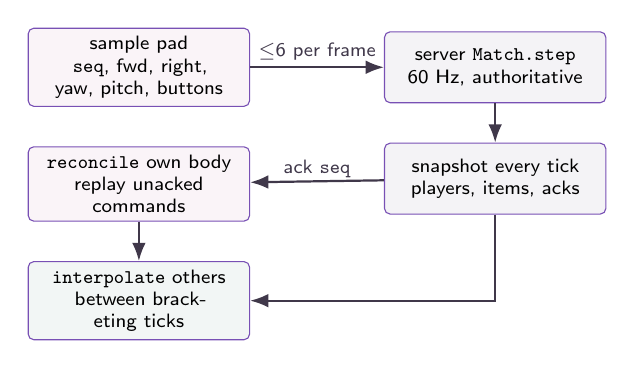
\begin{tikzpicture}[>=Latex,node distance=5mm,
 box/.style={draw=acpurple,rounded corners=2pt,align=center,font=\sffamily\scriptsize,minimum height=9mm,text width=26mm,inner sep=3pt},
 flow/.style={->,thick,draw=acdark},
 lbl/.style={font=\sffamily\scriptsize,text=acdark,inner sep=1pt}]
\node[box,fill=acpink!6] (input) {sample pad\\\code{seq}, fwd, right, yaw, pitch, buttons};
\node[box,right=17mm of input,fill=aclightgray] (server) {server \code{Match.step}\\60 Hz, authoritative};
\node[box,below=of server,fill=aclightgray] (snap) {snapshot every tick\\players, items, acks};
\node[box,below=of input,fill=acpink!6] (recon) {\code{reconcile} own body\\replay unacked commands};
\node[box,below=of recon,fill=acgreen!6] (interp) {\code{interpolate} others\\between bracketing ticks};
\draw[flow] (input) -- node[lbl,above=1pt] {$\le$6 per frame} (server);
\draw[flow] (server) -- (snap);
\draw[flow] (snap) -- node[lbl,above] {ack \code{seq}} (recon);
\draw[flow] (snap.south) |- (interp.east);
\draw[flow] (recon) -- (interp);
\end{tikzpicture}
\caption{dool's loop. Commands go up, snapshots come down; the client predicts only its own body from commands the server has not yet acknowledged and interpolates everyone else.}
\label{fig:dool}
\end{figure}

\section{What the tests said today}\label{sec:evidence}
Three suites were run on November 8, 2026 on one Mac with Node 24.22.1, against core revision \code{f2d1f744c2}, vault revision \code{0cedfd08} (oskiewar build 462) and the committed dool sources. Table~\ref{tab:suites} gives the counts. The relay suite and dool's suite are clean. The rollback suite is not, and the shape of its failures matters more than the count.

\begin{table}[t]
\centering\small
\begin{tabularx}{\columnwidth}{@{}L r r r@{}}
\toprule
suite & tests & pass & fail \\
\midrule
relay: \code{oskiewar-live-manager.test.mjs} & 43 & 43 & 0 \\
dool: \code{duel/test}, 12 files & 64 & 64 & 0 \\
rollback: \code{oskiewar-netplay.test.mjs} & 42 & 26 & 16 \\
\bottomrule
\end{tabularx}
\caption{Test record, November 8, 2026. The rollback suite runs two seats in one process over a fake wire with delay, jitter and loss.}
\label{tab:suites}
\end{table}

\subsection{Rollback: what passed}
Every assertion that is about synchronization passed: a snapshot restores the sim exactly and the same pads reproduce the same state; two seats fed the same pads over a laggy wire stay one fight; each seat measures its own round trip from the rival's echo; a seat that stops hearing the rival waits instead of guessing forever; equal clocks keep 60~Hz across a seven-frame wire; lead exchange bounds a faster peer without throttling equal ones; a desync drops both seats to the lane with one authority; a packet from the fight before is not played into this one; a revolver fight with shooting, emptying and throwing stays one fight across a sixteen-second lossy run; networked skatepark ropes converge after delayed grab, climb and swing inputs; a round is not filed until its end can no longer be taken back. The relay-side test that the rollback lane's packets pass seat to seat and never reach the grandstand, and that inputs take the datagram lane once both seats present their tokens, passed in the relay suite.

\subsection{Rollback: what failed, and why it is not the netcode}
The three long soak tests (\emph{SLOW MOTION}, \emph{AIR DROP}, \emph{UNARMED} \emph{remain synchronized through 25 seconds of delayed inputs and unequal paints}) ran 1,560 frames each with zero desyncs asserted on every frame on both seats, equalized, and matched state hashes, then failed on the final line: \code{roundState().map} now reads \code{DOJO} where the fixture expected the modifier's name. The game changed what that field reports; the fight stayed in step. The ninety-second \emph{TIME} deadline test fails because versus rounds are now untimed and the round never ends. Four gun-arena tests fail at the same jump (\emph{a jump at the crest takes the revolver}), one sword test reports that no blade was ever picked up, one coach test asks for two spawn columns the fixture map no longer has, two opening tests expect a fight to begin on a bare pad where the game now waits in \code{versus-lobby}, and the recording tests expect a round deadline that versus rounds no longer carry. All sixteen are fixtures reading game rules the game no longer follows. They are not a regression since the test file's last edit: the suite extracted at that commit (\code{c276173f}, November 5), run against that revision's engine with two helper modules the archive lacked linked from the current tree, fails the same sixteen by name. The fixtures were red when they were last committed. They should be repaired or retired, and an honest reviewer should hold the suite to that; but the property the suite exists to pin, that two machines fed the same inputs compute the same fight, held on every path that reached the assertion.

\subsection{What was not run}
The two-browser harness (\code{netplay-browser.mjs}) and the production fight harness were not run today: headless Chrome is not run on this Mac, and the browser harness needs one browser per seat. The last production verification on record, three fights on oskiewar.com with a wire tap on both pages, reconciled every state hash offline with zero mismatches and a deepest rollback of seven frames against the cap of eight \citep{multiplayer}. No cross-engine fight (browser against the native QuickJS console) has been proven, and the design expects it to desync: transcendental functions differ across engines and limb poses collide. Timing probes from this Mac to both relays returned TCP connects over two seconds to either host and were discarded as a measurement of the relays; the 64~ms against 193~ms figure stands on the October 14 measurement between two fleet machines \citep{westcoast}.

\section{Questions for a reviewer}\label{sec:questions}
This report exists to be handed to a peer, and these are the places a second pair of eyes would help most.
\begin{enumerate}
\item \textbf{Trust at the relay.} The datagram token is 96 random bits presented in cleartext over UDP, bound to a socket for the life of that socket, and trusted for 1.5~s after it last spoke. Is replaying a captured token within that window a problem worth closing, given that the relay only ever sends to an endpoint that has already spoken?
\item \textbf{Relay placement.} Two relays are listed in the client; there is no directory, and a room's relay is whichever the host reached fastest. Is a third copy on a club box worth standing up, and would the deploy script survive a Raspberry Pi behind a rathole tunnel, where UDP cannot be exposed?
\item \textbf{Desync repair.} Dropping to the streamed lane is honest but costs the rollback lane's latency for the rest of the fight. The 2~KiB channel is too small to carry a state resync. Is a one-time larger \code{resync} on the socket, with the host's snapshot as authority, worth the second code path?
\item \textbf{Cross-engine determinism.} Fixed-point or table-driven trigonometry for limb poses would let a browser fight a console. Is that worth doing before Steam, or is same-engine-only an acceptable rule for a game whose live routes are web and Apple?
\item \textbf{dool near the players.} dool's model does not need to change for a west-coast host; it needs an authority with the room's persistent store under it. Should that be a second lith, a Jamsocket session backend, or the oskiewar relay pattern with a store?
\item \textbf{The sixteen fixtures.} Should drifted gameplay fixtures be repaired, retired, or moved out of the netplay suite so that a red suite means a sync fault?
\end{enumerate}

\section{Ethics, privacy and limits}\label{sec:limits}
The relay forwards opaque packets between two seats that both chose the room; it validates shape and size and reads none of the game's words. Handles cross the wire only when a signed-in player sends them, and a guest is named by the line. The San Francisco health counters quoted above are aggregate lane statistics with no per-player content. The test record is one machine, one Node version, one day; the production numbers are cited, not reproduced. Nothing in this report is a security review, and the token question above is raised rather than answered.

\section{Conclusion}\label{sec:conclusion}
Oskiewar moves a fight by moving inputs through a relay that is deliberately dumb and deliberately near, and by making the simulation a pure function the relay never has to understand. dool moves a room by keeping one authority and letting the client guess only about itself. Both are small enough to read, both have suites that pin the property they depend on, and today those suites say the synchronization holds while sixteen gameplay fixtures have drifted away from the game. The open questions are about trust, placement and repair, which is where a peer's input would count.

\balance
\bibliographystyle{plainnat}
\bibliography{references}
\end{document}
